\documentclass[a4paper]{article}
\usepackage{graphicx,subcaption}
\usepackage{amsmath,amsfonts}
\usepackage{qtree}
\usepackage{tikz}
\title{Notes on Sequence Modelling}
\author{G.A. Jarrad}
\begin{document}
\maketitle
\numberwithin{equation}{section}
\numberwithin{figure}{section}
\numberwithin{table}{section}
\section{Introduction}\label{sec:intro}
blah, blah, blah

\section{Random Sequence Processes}
\label{sec:random-processes}
Consider a random process $\vec{R}=(R_1,R_2,R_3,\ldots)$ that generates arbitrary sequences of values
of the form $\vec{r}_n=(r_1,r_2,\ldots,r_n)$, where the length of any particular sequence is 
determined by a random variable $N$,
and the random variable $R_t$ denotes the $t$-th discrete stage in the sequence.
We assume that each $R_t$ randomly takes some discrete or continuous value $r_t\in{\cal R}$,
and hence the probability (or probability density) of observing a particular
sequence $\vec{r}_n$ of length $n$ is given by
\begin{eqnarray}
   p(\vec{R}=\vec{r}_n) & = & p(N=n)\; p(\vec{R}=\vec{r}_n\,|\,N=n)\,,
\end{eqnarray}
where
\begin{eqnarray}
p(\vec{R}=\vec{r}_n\,|\,N=n)
& = & p(\vec{R}_n=\vec{r}_n)~=~p(R_1=r_1,\ldots,R_n=r_n)\,.
\end{eqnarray}
In practice, this definition presupposes that we know we have a {\em complete} sequence that was initiated
at stage 1 and terminated at stage $n$.
Suppose instead that the sequence $\vec{r}_n$ was observed one stage at a time. How do we know if the
underlying process has actually terminated, or will instead
continue to generate another observed value
$r_{n+1}$, leading to the extended sequence $\vec{r}_{n+1}$? 
Similarly, how do we know that the first observed value $r_1$ was not in fact
part of a longer, unobserved sequence of values $(\ldots,r_0,r_1,\ldots)$?

In order to handle such difficulties, we consider any arbitrary sequence $\vec{r}_n$ to be {\em incomplete},
and explicitly denote the corresponding, complete sequence as $\langle\vec{r}_n\rangle$.
Additionally, we introduce the notion of {\em partially complete} sequences, 
defining a {\em start sequence} to be a sequence that has a definite start but an indefinite end,
denoted by $\langle\vec{r}_n]$, and futher defining an {\em end sequence} to be a sequence
that has a definite end but an indefinite start, denoted by $[\vec{r}_n\rangle$.

Under this augmented notation, knowledge about the start of a sequence can be encapsulated in 
a random indicator variable $\iota_0$, which takes on the value 1 if $R_1$ is definitely the first stage in the
sequence, or the value 0 if it is not. Similarly, the random indicator variable $\tau_{n+1}$
takes on the value 1 if $R_n$ is definitely the last stage in the sequence, or the value 0 if it is not.
Notionally, these indicators can be thought to correspond to pseudo-stages 0 and $N+1$, such that
the sequence is initiated at stage 0 and terminated at stage $N+1$.
This augmented random process is depicted in Figure~\ref{fig:random-process}.
\begin{figure}[hbt]
\centering
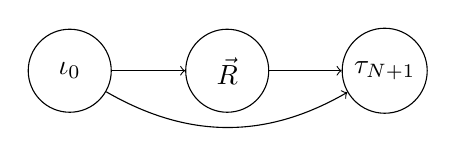
\begin{tikzpicture}[every node/.style={draw,circle,minimum size=3em,inner sep=3pt}]
    \node (1) at (0,0) {$\iota_0$};
    \node (2) at (2, 0)  {$\vec{R}$};
    \node (3) at (4, 0) {$\tau_{N+1}$};

    \draw[->] (1) edge (2) ;
    \draw[->] (1) to[out=-30,in=-150] (3) ;
    \draw[->] (2) edge (3) ;
\end{tikzpicture}
\caption{A random process for generating both complete and incomplete sequences of random length $N$,
with explicit stages for sequence initiation and termination.}
\label{fig:random-process}
\end{figure}

The probability of a given complete sequence $\langle\vec{r}_n\rangle$ is now defined as
\begin{eqnarray}
   p(\langle\vec{r}_n\rangle)
& = & p(\iota_0=1,R_1=r_1\ldots,R_n=r_n,\tau_{n+1}=1)
\,,
\end{eqnarray}
such that $p(N=n)\equiv p(\iota_0=1,\tau_{n+1}=1)$.
Likewise, the probability
of a given start sequence $\langle\vec{r}_n]$ is defined as
\begin{eqnarray}
p(\langle\vec{r}_n]) & = & p(\iota_0=1,R_1=r_1\ldots,R_n=r_n)\,,
\end{eqnarray}
and the probability of the end sequence $[\vec{r}_n\rangle$ is
\begin{eqnarray}
p([\vec{r}_n\rangle)
& = & p(R_1=r_1\ldots,R_n=r_n,\tau_{n+1}=1)\,.
\end{eqnarray}
In the special case where we know in advance that a start sequence definitely does not terminate
at stage $n+1$ (i.e.\ $\tau_{n+1}=0$),  we may instead write
\begin{eqnarray}
p(\langle\vec{r}_n!)
& = & p(\iota_0=1,R_1=r_1\ldots,R_n=r_n,\tau_{n+1}=0)\,.
\end{eqnarray}
Likewise, if an end sequence definitely does not initiate at stage
0 (i.e.\ $\iota_0=0$), then
\begin{eqnarray}
p(!\vec{r}_n\rangle)
& = & p(\iota_0=0,R_1=r_1\ldots,R_n=r_n,\tau_{n+1}=1)\,.
\end{eqnarray}
The four remaining types of sequences, namely $[\vec{r}_n]$, $!\vec{r}_n]$, $[\vec{r}_n!$ and $!\vec{r}_n!$ , can be similarly defined.

%%%%%%%%%%%%%%%%%%%%%%%%%%%%%%%%%%%
\section{Markov Sequence Processes}
\label{sec:markov-processes}
In Section~\ref{sec:random-processes} we defined a random process $\vec{R}$ and the sequences it generates.
We now assume that the process is also {\em causal}, meaning that each stage of a sequence,
including the initiation stage and the termination stage, depends only on the preceding stages.
Hence, under the Markov assumption of conditional independence,
the process depicted in Figure~\ref{fig:random-process} leads to the conditional model
\begin{eqnarray}
\!\!\!\!\!\!p(\langle\vec{r}_n\rangle)
&\!\!=\!\!& p(\iota_0=1)\;p(\vec{R}_n=\vec{r}_n\,|\,\iota_0=1)\;
p(\tau_{n+1}=1\:|\;\iota_0=1,\vec{R}_n=\vec{r}_n)
\,.
\end{eqnarray}
We can further decompose the model for $\vec{R}$, since the distribution of
values for variable $R_t$, at stage $t$, depends directly upon the values generated previously
in the sequence at stages $t-1,t-2,\ldots,1$. 
This expanded causal process is depicted in Figure~\ref{fig:causal-process}.
\begin{figure}[hbt]
\centering
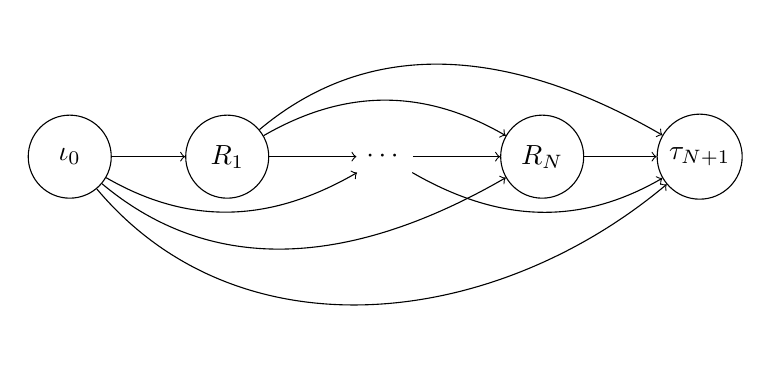
\begin{tikzpicture}[cnode/.style={draw,circle,minimum size=3em,inner sep=3pt}]
    \node[cnode] (0) at (0,0) {$\iota_0$};
    \node[cnode] (1) at (2,0) {$R_1$};
    \node (any) at (4,0) {$\cdots$};
    \node[cnode] (n) at (6, 0)  {$R_N$};
    \node[cnode] (np1) at (8, 0) {$\tau_{N+1}$};

    \draw[->] (0) edge (1) ;
    \draw[->] (0) to[out=-30,in=-150] (any) ;
    \draw[->] (0) to[out=-40,in=-150] (n) ;
    \draw[->] (0) to[out=-50,in=-140] (np1) ;

    \draw[->] (1) edge (any) ;
    \draw[->] (1) to[out=30,in=150] (n) ;
    \draw[->] (1) to[out=40,in=150] (np1) ;

    \draw[->] (any) edge (n) ;
    \draw[->] (any) to[out=-30,in=-150] (np1) ;

    \draw[->] (n) edge (np1) ;
\end{tikzpicture}
\caption{A fully-connected causal process for generating temporal sequences of random length $N$.}
\label{fig:causal-process}
\end{figure}
Hence, the probability of a complete, causal sequence is taken here to be
\begin{eqnarray}
p(\langle\vec{r}_{n}\rangle)
& = & 
p(\iota_0=1)\;
\prod_{t=1}^{n}
p(R_t=r_t\,|\,\vec{R}_{t-1}=\vec{r}_{t-1},\iota_0=1)
\nonumber\\&&
p(\tau_{n+1}=1\,|\,\vec{R}_{n}=\vec{r}_{n},\iota_0=1)
\,.
\label{eq:temporal-model}
\end{eqnarray}

The related models for partially complete or incomplete sequences can be similarly obtained
by suitably modifying the corresponding boundary conditions for $\iota_0$ and $\tau_{n+1}$
--- refer to Section~\ref{sec:random-processes}.
In general, all types of sequences can be handled by a slight change of notation.
Let $V$ denote an arbitrary node variable, such that $V_0=\iota_0$, $V_t=R_t$ for $t=1,2,\ldots,N$,
and $V_{N+1}=\tau_{N+1}$, and consider $\vec{V}=(V_0,\ldots,V_{N+1})$. 
Likewise, let $\vec{v}$ denote an observed sequence of values, e.g.\ $\vec{v}=\langle\vec{r}_n\rangle$, or
$\vec{v}=[\vec{r}_n\rangle$, et cetera. Then the causal process model~\eqref{eq:temporal-model} reduces to
\begin{eqnarray}
p(\vec{v}) & = & \prod_{t=0}^{n+1}p(V_t=v_t\,|\,\vec{\Pi}_t(\vec{V})=\vec{\pi}_t(\vec{v}))\,,
\end{eqnarray}
where $\vec{\Pi}_t(\vec{V})=(V_0,V_1,\ldots,V_{t-1})$ denotes the predecessor nodes upon which node $V_t$
is conditionally dependent, and 
$\vec{\pi}_t(\vec{v})=(v_0,v_1,\ldots,v_{t-1})$ similarly denotes the observed values of those predecessor nodes. 

In practice, the causal model is usually simplified further by limiting the 
conditional dependency on past values to a maximum number $m$ of terms.
Hence, this so-called {\em $m$-th order Markov model} is given by
\begin{eqnarray}
p(\vec{v}) & = & \prod_{t=0}^{n+1}p(V_t=v_t\,|\,\vec{\Pi}^{(m)}_t(\vec{V})=\vec{\pi}_t^{(m)}(\vec{v}))\,,
\end{eqnarray}
where the predecessor nodes are now given by
\begin{eqnarray}
\vec{\Pi}_t^{(m)}(\vec{V}) & = & 
\left\{
\begin{array}{ll}
(V_0,V_1,\ldots,V_{t-1}) & \mbox{if }t\le m\,,
\\
(V_{t-m},V_{t-m+1},\ldots,V_{t-1}) & \mbox{if }t>m
\end{array}
\right.\,.
\end{eqnarray}
An example from the realm of natural language understanding is the lexicographical analysis of the character
sequences of words using bigrams (pairs of adjacent characters, corresponding to $m=1$), and trigrams 
(triples of adjacent characters, corresponding to $m=2$), et cetera.

In the special case of $m=1$, the first-order Markov model takes on the even simpler form
\begin{eqnarray}
p(\vec{v}) & = & \prod_{t=0}^{n+1}p(V_t=v_t\,|\,V_{t-1}=v_{t-1})\,,
\end{eqnarray}
or, closer to the original notation:
\begin{eqnarray}
\!\!p(\iota_0,\vec{r}_n,\tau_{n+1}) & = & 
p(\iota_0)p(R_1=r_1\,|\,\iota_0)
\prod_{t=2}^{n}p(R_t=r_t\,|\,R_{t-1}=r_{t-1})
\nonumber\\&&
p(\tau_{n+1}\,|\,R_n=r_n)
\,.
\end{eqnarray}
This process is depicted in Figure~\ref{fig:markov-1-process}, and will henceforth be taken as the basis of our analyses.
\begin{figure}[hbt]
\centering
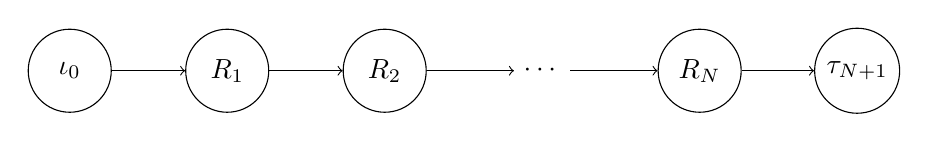
\begin{tikzpicture}[cnode/.style={draw,circle,minimum size=3em,inner sep=3pt}]
    \node[cnode] (0) at (0,0) {$\iota_0$};
    \node[cnode] (1) at (2,0) {$R_1$};
    \node[cnode] (2) at (4,0) {$R_2$};
    \node (any) at (6,0) {$\cdots$};
    \node[cnode] (n) at (8, 0)  {$R_N$};
    \node[cnode] (np1) at (10, 0) {$\tau_{N+1}$};

    \draw[->] (0) edge (1) ;
    \draw[->] (1) edge (2) ;
    \draw[->] (2) edge (any) ;
    \draw[->] (any) edge (n) ;
    \draw[->] (n) edge (np1) ;
\end{tikzpicture}
\caption{A first-order Markov process for generating causal sequences of random length $N$.}
\label{fig:markov-1-process}
\end{figure}

\section{Stateful Markov Sequence Processes}
Consider the first-order Markov process $\vec{R}$ depicted in Figure~\ref{fig:markov-1-process}.
Suppose now that the random variable $R_t$ at stage $t$ can be decomposed into the tuple
$R_t=(S_t,X_t)$, where $S_t$ is a discrete random variable taking values $s_t\in{\cal S}$, and $X_t$
is a discrete or continuous random variable taking values $x_t\in{\cal X}$.
We may call $S_t$ the {\em state} of the process at stage $t$, and $X_t$ its {\em value}.
The joint state--value model then takes the form 
\begin{eqnarray}
p(\iota_0,\vec{S}_n,\vec{X}_n,\tau_{n+1}) & = & 
p(\iota_0)\,p(S_1,X_1\,|\,\iota_0)
\nonumber\\&&
\prod_{t=2}^{n}p(S_t,X_t\,|\,S_{t-1},X_{t-1})
p(\tau_{n+1}\,|\,S_n,X_n)
\,,
\end{eqnarray}
corresponding to the {\em stateful} process is depicted in Figure~\ref{fig:stateful-1-process}.
\begin{figure}[hbt]
\centering
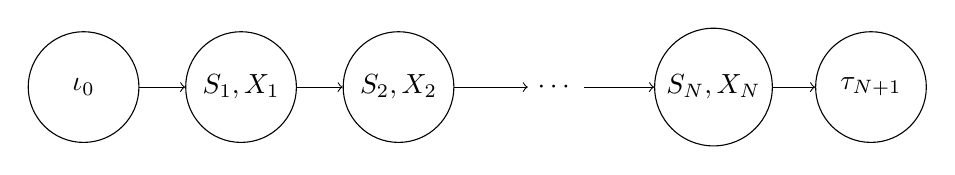
\begin{tikzpicture}[cnode/.style={draw,circle,minimum size=4em,inner sep=3pt}]
    \node[cnode] (0) at (0,0) {$\iota_0$};
    \node[cnode] (1) at (2,0) {$S_1, X_1$};
    \node[cnode] (2) at (4,0) {$S_2, X_2$};
    \node (any) at (6,0) {$\cdots$};
    \node[cnode] (n) at (8, 0)  {$S_N, X_N$};
    \node[cnode] (np1) at (10, 0) {$\tau_{N+1}$};

    \draw[->] (0) edge (1) ;
    \draw[->] (1) edge (2) ;
    \draw[->] (2) edge (any) ;
    \draw[->] (any) edge (n) ;
    \draw[->] (n) edge (np1) ;
\end{tikzpicture}
\caption{A first-order Markov process for generating stateful sequences of random length $N$.}
\label{fig:stateful-1-process}
\end{figure}

We now impose futher structure on the process by specifying the relationship within stage $t$,
and also expanding on the relationship between stage $t$ and stage $t+1$.
Firstly, it is commonly supposed that the process determines the state $S_t$ based on available information,
and then from $S_t$ selects the value $X_t$.
Next, in the general case both $S_{t+1}$ and $X_{t+1}$ may depend upon $S_t$ and $X_t$. 
Hence, the structured stateful model is now given by
\begin{eqnarray}
p(\iota_0,\vec{S}_n,\vec{X}_n,\tau_{n+1}) & = & 
p(\iota_0)\,p(S_1\,|\,\iota_0)\,p(X_1\,|\,S_1,\iota_0)
\nonumber\\&&
\prod_{t=2}^{n}p(S_t\,|\,S_{t-1},X_{t-1})
\,p(X_t\,|\,S_t,S_{t-1},X_{t-1})
\nonumber\\&&
p(\tau_{n+1}\,|\,S_n,X_n)
\,,
\end{eqnarray}
corresponding to the process is depicted in Figure~\ref{fig:gen-stateful-1-process}.
\begin{figure}[hbt]
\centering
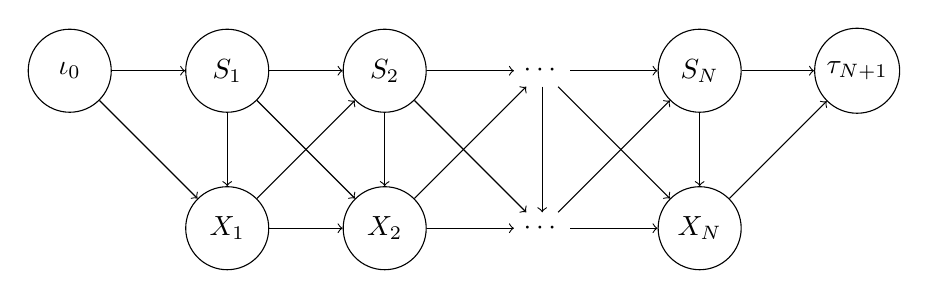
\begin{tikzpicture}[cnode/.style={draw,circle,minimum size=3em,inner sep=3pt}]
    \node[cnode] (0) at (0,0) {$\iota_0$};
    \node[cnode] (1) at (2,0) {$S_1$};
    \node[cnode] (1x) at (2,-2) {$X_1$};
    \node[cnode] (2) at (4,0) {$S_2$};
    \node[cnode] (2x) at (4,-2) {$X_2$};
    \node (t) at (6,0) {$\cdots$};
    \node (tx) at (6,-2) {$\cdots$};
    \node[cnode] (n) at (8, 0)  {$S_N$};
    \node[cnode] (nx) at (8, -2)  {$X_N$};
    \node[cnode] (np1) at (10, 0) {$\tau_{N+1}$};

    \draw[->] (0) edge (1) ;
    \draw[->] (0) edge (1x) ;
    \draw[->] (1) edge (1x) ;
    \draw[->] (1) edge (2) ;
    \draw[->] (1) edge (2x) ;
    \draw[->] (1x) edge (2) ;
    \draw[->] (1x) edge (2x) ;
    \draw[->] (2) edge (2x) ;
    \draw[->] (2) edge (t) ;
    \draw[->] (2) edge (tx) ;
    \draw[->] (2x) edge (t) ;
    \draw[->] (2x) edge (tx) ;
    \draw[->] (t) edge (tx) ;
    \draw[->] (t) edge (n) ;
    \draw[->] (t) edge (nx) ;
    \draw[->] (tx) edge (n) ;
    \draw[->] (tx) edge (nx) ;
    \draw[->] (n) edge (nx) ;
    \draw[->] (n) edge (np1) ;
    \draw[->] (nx) edge (np1) ;
\end{tikzpicture}
\caption{A general interpretation of the first-order stateful Markov process for generating sequences of random length $N$.}
\label{fig:gen-stateful-1-process}
\end{figure}

It is more usual, however, to further restrict the complexity of the process 
by also imposing the first-order Markov assumption at the level
of the state--value transitions themselves, leading to the restricted stateful  model
\begin{eqnarray}
p(\iota_0,\vec{S}_n,\vec{X}_n,\tau_{n+1}) & = & 
p(\iota_0)\,p(S_1\,|\,\iota_0)\,p(X_1\,|\,S_1,\iota_0)
\nonumber\\&&
\prod_{t=2}^{n}p(S_t\,|\,S_{t-1})
\,p(X_t\,|\,S_t)
\nonumber\\&&
p(\tau_{n+1}\,|\,S_n)
\,,
\label{eq:1-stateful-markov-model}
\end{eqnarray}
with the corresponding process shown in Figure~\ref{fig:1-stateful-1-process}.
\begin{figure}[hbt]
\centering
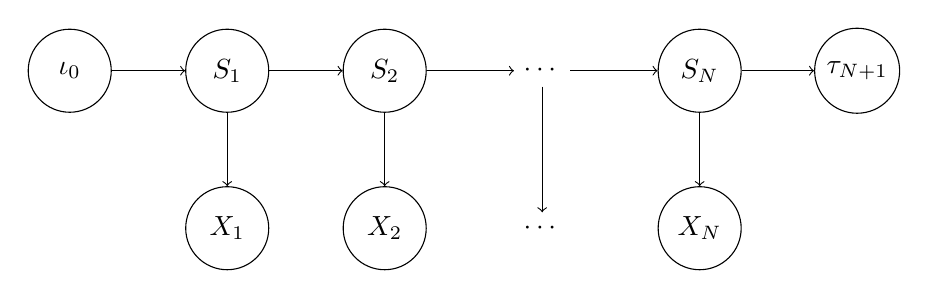
\begin{tikzpicture}[cnode/.style={draw,circle,minimum size=3em,inner sep=3pt}]
    \node[cnode] (0) at (0,0) {$\iota_0$};
    \node[cnode] (1) at (2,0) {$S_1$};
    \node[cnode] (1x) at (2,-2) {$X_1$};
    \node[cnode] (2) at (4,0) {$S_2$};
    \node[cnode] (2x) at (4,-2) {$X_2$};
    \node (t) at (6,0) {$\cdots$};
    \node (tx) at (6,-2) {$\cdots$};
    \node[cnode] (n) at (8, 0)  {$S_N$};
    \node[cnode] (nx) at (8, -2)  {$X_N$};
    \node[cnode] (np1) at (10, 0) {$\tau_{N+1}$};

    \draw[->] (0) edge (1) ;
    \draw[->] (1) edge (1x) ;
    \draw[->] (1) edge (2) ;
    \draw[->] (2) edge (2x) ;
    \draw[->] (2) edge (t) ;
    \draw[->] (t) edge (tx) ;
    \draw[->] (t) edge (n) ;
    \draw[->] (n) edge (nx) ;
    \draw[->] (n) edge (np1) ;
\end{tikzpicture}
\caption{A restricted interpretation of the first-order stateful Markov process for generating sequences of random length $N$.}
\label{fig:1-stateful-1-process}
\end{figure}

\section{Hidden-state Markov Sequence Processes}

Consider the stateful, first-order Markov process depicted by Figure~\ref{fig:1-stateful-1-process}.
Suppose now that the value of state $S_t$ at any stage $t$ is never observed, only the value of $X_t$.
Then the model~\eqref{eq:1-stateful-markov-model} may be considered to be a {\em hidden-state} Markov model (or HMM).
As such, the state of $S_t$ must be deduced from knowledge of the observed sequence $\vec{x}_n$. This is accomplished
via the forward--backward algortithm. The forward step commences with stages $0$ and $1$, by defining
\begin{eqnarray}
  \alpha_1(s_1) & = & p(\iota_0,x_1,s_1)
\nonumber\\
& = & p(\iota_0)\,p(S_1=s_1\,|\,\iota_0)\,p(X_1=x_1\,|\,S_1=s_1)
\nonumber\\
& = & p(\iota_0)\,p(s_1\,|\,\iota_0)\,p(x_1\,|\,s_1)
\,,
\end{eqnarray}
from equation~\eqref{eq:1-stateful-markov-model}, where the explicit variables $S_t$ and $X_t$ may now be
dropped for convenience when the context is unambiguous.
Then it follows that
\begin{eqnarray}
  \alpha_2(s_2) & = & p(\iota_0,x_1,x_2,s_2)
\nonumber\\
& = & \sum_{s_1\in{\cal S}}p(\iota_0,x_1,s_1)\,p(s_2\,|\,s_1)\,p(x_2\,|\,s_2)
\nonumber\\
& = & \sum_{s_1\in{\cal S}}\alpha_1(s_1)\,p(s_2\,|\,s_1)\,p(x_2\,|\,s_2)\,,
\end{eqnarray}
and in general that
\begin{eqnarray}
   \alpha_t(s_t) & = & p(\iota_0,\vec{x}_t,s_t)
\nonumber\\
& = & \left\{\sum_{s_{t-1}\in{\cal S}}\alpha_{t-1}(s_{t-1})\,p(s_t\,|\,s_{t-1})\right\}\,p(x_t\,|\,s_t)\,,
\end{eqnarray}
for $t=2,3,\ldots,n$.
Consequently, we may predict $S_t$ from a partially observed sequence $\vec{x}_t$ via
\begin{eqnarray}
  p(s_t\,|\,\iota_0,\vec{x}_t) & = & \frac{p(\iota_0,\vec{x}_t,s_t)}{p(\iota_0,\vec{x}_t)}
~=~\frac{\alpha_t(s_t)}{\sum_{s_t'\in{\cal S}}\alpha_t(s_t')}\,.
\end{eqnarray}
Similarly, we may predict the next observation $X_{t+1}$ via
\begin{eqnarray}
  p(x_{t+1}\,|\,\iota_0,\vec{x}_t) 
& = &
  \frac{p(\iota_0,\vec{x}_t,x_{t+1})}{p(\iota_0,\vec{x}_t)}
\nonumber\\
& = & 
 \frac{\sum_{s_{t+1}\in{\cal S}}\sum_{s_{t}\in{\cal S}}p(\iota_0,\vec{x}_t,s_t)\,p(s_{t+1}\,|\,s_t)\,p(x_{t+1}\,|\,s_{t+1})}
        {p(\iota_0,\vec{x}_t)}
\nonumber\\
& = &
  \frac{\sum_{s_{t+1}\in{\cal S}}\sum_{s_{t}\in{\cal S}}\alpha_t(s_t)\,p(s_{t+1}\,|\,s_t)\,p(x_{t+1}\,|\,s_{t+1})}{\sum_{s_t\in{\cal S}}\alpha_t(s_t)}\,.
\end{eqnarray}

The backward step now commences with stage $n+1$, by defining
\begin{eqnarray}
  \beta_{n}(s_{n}) & = & p(\tau_{n+1}\,|\,s_{n})
\,,
\end{eqnarray}
and 
\begin{eqnarray}
  \beta_{n-1}(s_{n-1}) & = & p(x_{n},\tau_{n+1}\,|\,s_{n-1})
\nonumber\\
& = &
\sum_{s_n\in{\cal S}}p(\tau_{n+1}\,|\,s_{n})\,p(x_n\,|\,s_n)\,p(s_n\,|\,s_{n-1})
\nonumber\\
& = &
\sum_{s_n\in{\cal S}}\beta_n(s_{n})\,p(x_n\,|\,s_n)\,p(s_n\,|\,s_{n-1})
\,.
\end{eqnarray}
In general, we recursively define
\begin{eqnarray}
  \beta_{t}(s_{t}) & = & p(x_{t+1},\ldots,x_{n},\tau_{n+1}\,|\,s_{t})
\nonumber\\
& = &
\sum_{s_{t+1}\in{\cal S}}
  p(x_{t+2},\ldots,x_{n},\tau_{n+1}\,|\,s_{t+1})\,p(x_{t+1}\,|\,s_{t+1})\,p(s_{t+1}\,|\,s_t)
\nonumber\\
& = &
\sum_{s_{t+1}\in{\cal S}}\beta_{t+1}(s_{t+1})\,p(x_{t+1}\,|\,s_{t+1})\,p(s_{t+1}\,|\,s_t)
\,.
\end{eqnarray}
Consequently, we may now calculate the probability of an entirely observed sequence $\vec{x}_n$ as
\begin{eqnarray}
  p(\iota_0,\vec{x}_n,\tau_{n+1}) & = & 
  \sum_{s_n\in{\cal S}}p(\iota_0,\vec{x}_n,s_n)\,p(\tau_{n+1}\,|\,s_n)
\nonumber\\& = &
  \sum_{s_n\in{\cal S}}\alpha_n(s_n)\beta_n(s_n)\,,
\end{eqnarray}
and retrospectively predict $S_t$ given $\vec{x}_n$ via
\begin{eqnarray}
  p(s_t\,|\,\iota_0,\vec{x}_n,\tau_{n+1}) & = & 
\frac{p(\iota_0,\vec{x}_n,s_t,\tau_{n+1})}
       {p(\iota_0,\vec{x}_n,\tau_{n+1})}
\nonumber\\& = &
\frac{p(\iota_0,\vec{x}_t,s_t)\,p(x_{t+1},\ldots,x_n,\tau_{n+1}\,|\,s_t)}{p(\iota_0,\vec{x}_n,\tau_{n+1})}
\nonumber\\& = &
\frac{\alpha_t(s_t)\beta_t(s_t)}{\sum_{s_t'\in{\cal S}}\alpha_t(s_t')\beta_t(s_t')}\,.
\end{eqnarray}

%%%%%%%%%%%%%%%%%%%%%%%%%%%%%%%%%%%%
\end{document}
